\documentclass[a4paper, 10pt]{article}

\usepackage[T1]{fontenc}
\usepackage[utf8]{inputenc}
\usepackage[english]{babel}
\usepackage{fullpage}
\usepackage{graphicx}
\usepackage{caption}
\usepackage{float}
%\usepackage{layout}
%\usepackage{geometry}
%\usepackage{setspace}
%\usepackage{soul}
%\usepackage{ulem}
%\usepackage{eurosym}
%\usepackage{bookman}
%\usepackage{charter}
%\usepackage{newcent}
%\usepackage{lmodern}
%\usepackage{mathpazo}
%\usepackage{mathptmx}
\usepackage{url}
\usepackage{setspace}
%\usepackage{verbatim}
%\usepackage{moreverb}
%\usepackage[french, onelanguage, linesnumbered, ruled, vlined]{algorithm2e}
%\usepackage{listings}
%\usepackage{fancyhdr}
%\usepackage{wrapfig}
\usepackage{color}
%\usepackage{colortbl}
\usepackage{amsmath}
\usepackage{amssymb}
\usepackage{amsfonts}
\usepackage{amsthm}
%\usepackage{mathrsfs}
%\usepackage{makeidx}
\usepackage{parskip}
\usepackage{titlesec}
\usepackage{hyperref}
\usepackage[nottoc, notlof, notlot]{tocbibind}
%\usepackage{algorithm2e}
\DeclareMathOperator*{\argmax}{arg\,max}
\DeclareMathOperator*{\argmin}{arg\,min}

% Title Page
\title{CGDI Inpainting}
\author{Louis Béthune et Léonard Assouline}
\date{}

\begin{document}
\maketitle
\tableofcontents

\section{L'algorithme}

\subsection{Introduction}

Nous avons implémenté l'algorithme de \cite{newson2017non} tel qu'il est décrit dans leur article.  
  
Il s'agit d'un algorithme fonctionnant à base de "patchs" : ce sont des zones rectangulaires prises ailleurs dans l'image, qu'on va utiliser pour remplir l'occlusion de façon à minimiser une certaine distance afin de produire des recollements réalistes conformes à ce qui est observé ailleurs dans l'image.  
  
Nous n'allons pas décrire dans le détail cet algorithme (on vous renvoie à l'article original pour cela) mais nous allons le résumer.  

L'image complète sera désignée par $\Omega$, la zone non efface sera décrite par $\mathcal{D}$ et l'occlusion sera décrite par $\mathcal{H}$. Une position sera décrite par $p(x,y)$ et le contenu de l'image sera décrit par $u : \Omega\rightarrow \mathbb{R}^3$.  
Un patch est un voisinage rectangulaire d'un point : le voisinage de positions sera désigné $\mathcal{N}_p$ pour le point $p$, et le patch lui même sera désigné $W_p$.  
Notre objectif de déterminer le plus proche voisin d'un patch donné : pour une fonction de distance $d$ le plus proche voisin de $W_p$ est $W_q$ avec $q=\argmin d^2(W_p,W_q)$.  
    
Nous allons désigner par $\phi : \Omega \rightarrow \mathbb{N}^2$ la fonction qui à une position associe l'offset, c'est à dire la différence coordonnée à coordonnée, entre un point $p$ et son patch associé $p+\phi(p)$. Cette information sert de support à l'algorithme.  
  
\subsection{Approximate Nearest Neighbor}
  
Trouver le plus proche voisin est un problème difficile car une recherche exhaustive mène à des temps de calcul exagérément longs. Mais il existe une heuristique popularisé dans \cite{barnes2009patchmatch} permettant d'accélérer cette recherche à condition de sacrifier des garanties sur l'optimalité du résultat : en combinant une recherche aléatoire (exploration) et la propagation de "bons" patchs d'un pixel à un autre (exploitation).    

\begin{center}
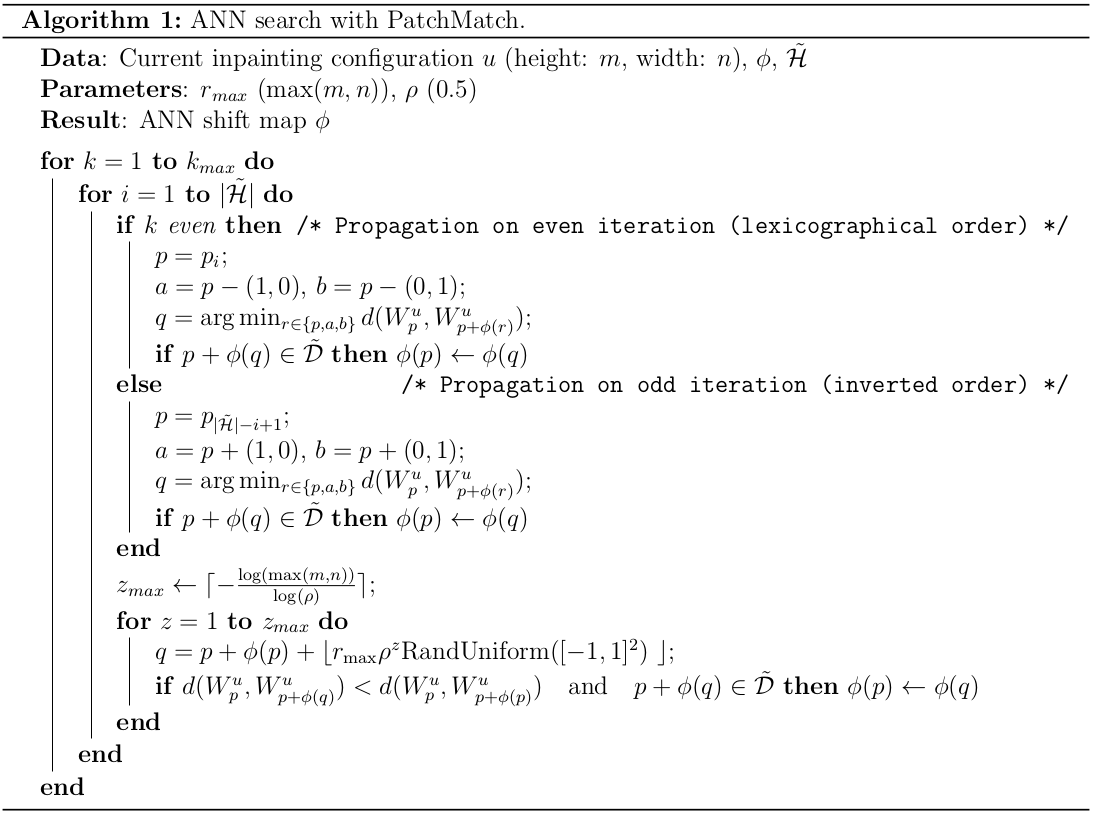
\includegraphics[scale=0.26]{ANN.png} 
\end{center}
  
\subsection{La reconstruction}

Une fois que de bons patchs candidats ont été trouvés il faut reconstruire l'image. Plein de méthodes, plus ou moins naïves, existent dans la littérature. Celle de l'article donne de bons résultats : chaque pixel est colorée avec une somme pondérée des couleurs des patchs auquel il appartient. Cette pondération dépend de la distance associée à ce patch, de façon à favoriser les couleurs des patchs appropriés à la zone à inpaintée.  
  
Cet algorithme est donné par les formules suivantes :

$$u(p)=\frac{\sum_{q\in\mathcal{N}_p} s_q^pu(p+\phi(q))}{\sum_{q\in\mathcal{N}_p} s_q^p}$$

Avec :

$$s_q^p=\exp{\frac{-d^2(W_q,W_{q+\phi(q)})}{2\sigma^2}}$$

Avec $\sigma$ choisi comme le 75ème percentile de toutes les distances. Cet algorithme tend à produire des images floues, ce qui n'est pas un problème lors des étapes intermédiaires. En revanche, sur l'étape de reconstruction finale, on n'effectue pas de moyenne pondérée : on garde la couleur du pixel dont la distance associée est la meilleure. On attend donc le dernier moment pour recoller des morceaux de patch entiers. Si on avait effectué cette opération plus tôt on aurait piégé l'algorithme dans un mauvais minimum local. Là, on s'assure de reproduire un résultat net et précis.

\subsection{La distance}

La distance est rarement discutée dans les articles du domaine. Une mesure évidente est la norme deux (prise au carré pour éviter les opérations coûteuses de calcul de racine), de la différence pixel à pixel de chaque patch sur chaque canal \textbf{RGB}. Mais cette mesure présente des défauts : elle est susceptible de confondre deux texture dont la couleur moyenne est semblable mais dont les "motifs" (comprendre : la structure) sont différents. Dans l'article original, on propose pour solution d’utiliser une \textit{texture feature map} $T$ pour comme terme supplémentaire pour régler ce problème : il s'agit d'un tableau contenant des valeurs calculées à partir des dérivées de l'image originale dans les directions $x$ et $y$. Il apparaît de façon heuristique que ce nouveau terme permet de lever l'ambiguïté sur les textures semblables, et augmente la qualité du résultat.  
  
$$d^2(W_p,W_q)=\frac{1}{N}\sum_{r\in\mathcal{N}_p}(\|u(r)-u(r-p+q)\|_2^2+\lambda\|T(r)-T(r-p+q)\|_2^2)$$

Avec : $$T(p)=\frac{1}{\textbf{card}(\nu)}\sum_{q\in\nu}(|I_x(q)|,|I_y(q)|)$$

Avec $I_x$ et $I_y$ les dérivées dans les directions $x$ et $y$ respectivement.  
  
Nous avons également testé d'autres distances, comme par exemple l'angle entre les deux patchs (chaque patch vu comme un vecteur). Cela n'a pas donné de résultats satisfaisants.

\subsection{La pyramide}

Cet algorithme utilise une pyramide gaussienne : c'est à dire qu'il construit une suite d'images par \textit{downsampling} successifs, complétés d'une interpolation gaussienne. Cette pyramide a une hauteur telle que dans l'image de résolution minimale, la taille de l'occlusion est du même ordre de grandeur que le patchsize. Cela permet de voir l'inpainting comme un procédé itératif : on commence par inpainter les images de faible résolution pour reconstruire de larges zones de l'image de façon cohérente, puis progressivement on \textit{upsample} le résultat obtenu pour affiner sa qualité et inpainter des détails de plus en plus précis (dans les images de haute résolution le patchsize est souvent petit devant la taille de l'occlusion). Se référer à l'article originel pour plus de détails.

\subsection{L'algorithme final}

\begin{center}
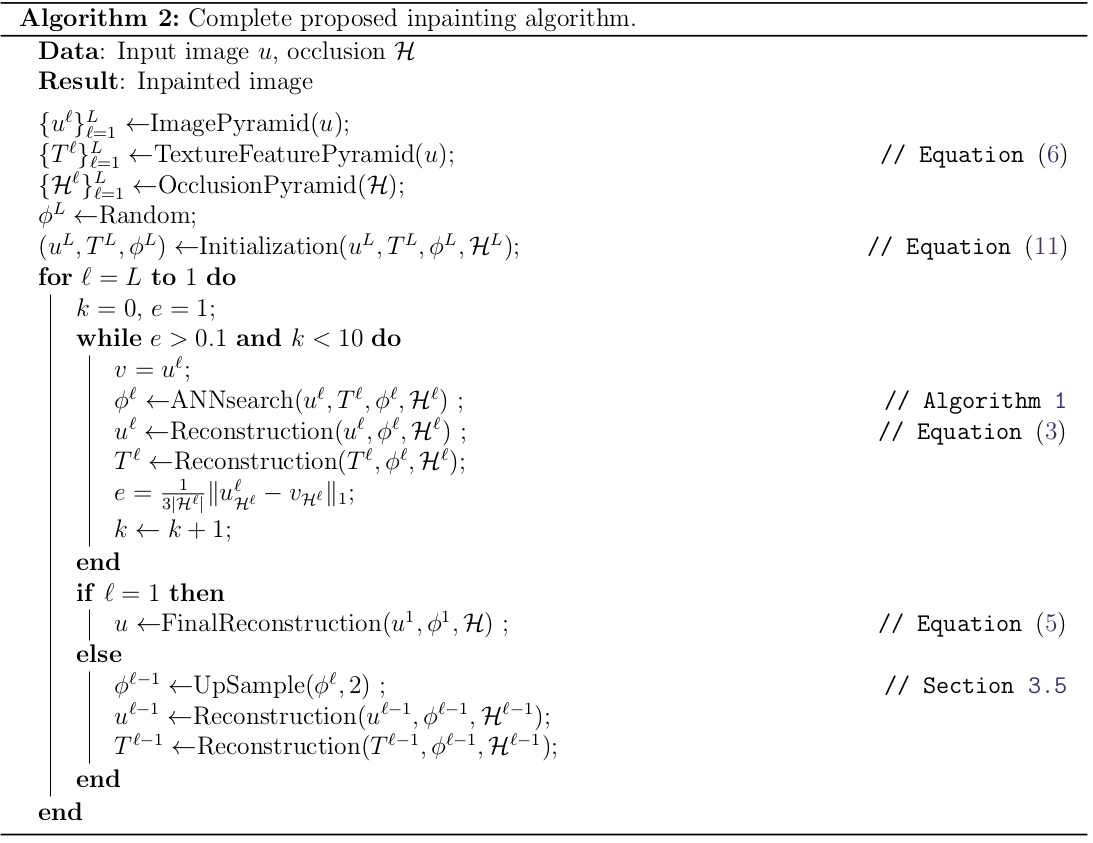
\includegraphics[scale=0.30]{inpainting_algo.png} 
\end{center}

\section{Implémentation}

\subsection{Le programme}

Le programme a été écrit en \textbf{C++14} et utilise les fonctionnalités d'\textbf{OpenCV} (version \textbf{3.1} et supérieur). Il y une dépendance avec Boost.Options, et les options disponibles peuvent être affichées en tapant \textbf{-h} ou \textbf{--help}.  
  
On peut fournir un masque avec l'option \textbf{-m} mais c'est optionnel. Si aucun masque n'est fourni une fenêtre va s'ouvrir et permet à l'utilisateur de créer son propre masque en cliquant dans l'image, régler la taille du pinceau avec les touches \textbf{+} ou \textbf{-}. Le masque créé apparaît alors en négatif. Si l'option \textbf{-c} est activée le masque sera enregistré sur le disque avec le nom fourni en argument.
  
L'option \textbf{-p} contrôle la taille des patchs. Il vaut mieux utiliser des entiers impairs. L'option \textbf{-l} permet de modifier $\lambda$, c'est à dire le tradeoff entre les distances pixel à pixel et la \textit{feature map}.
  
Le temps d'exécution dépend de plusieurs facteurs, parmi lesquels la taille de l'image, la taille de l'occlusion, et la taille des patchs (ce dernier paramètre peut, pour une même image grand format, faire varier le temps d'exécution de quelques secondes à presque une minute). L'option \textbf{-a} qui contrôle le nombre d'itérations de ANN peut servir à directement modifier le temps d'exécution, au prix d'une recherche de plus proches voisins plus ou moins efficace.  
  
Durant la production de l'image l'image va être successivement affichées en plusieurs dimensions (une pour chaque niveau de la pyramide) pour qu'on puisse suivre en temps réel l'inpainting. Aussi, il ne faut considérer l'inpainting comme terminé que lorsque "done" s'affiche dans la console.

\subsection{L'organisation du code}

Le fichier \textbf{cvui.h} est une librairie extérieure que nous n'avons pas codé. Les fichiers \textbf{gui\_squeleton} contiennent le code de l'éditeur de masque interactif. Les fichiers \textbf{inpainting} contiennent le squelette général de l'algorithme. Les fichier \textbf{ANNsearch} contiennent l'implémentation de l'algorithme ANN ainsi que quelques utilitaires pour manipuler des patchs ou des distances. Pour finir les fichiers \textbf{reconstruction} contiennent les codes de reconstruction et d'initialisation de l'image. Le total fait à peu près 600 lignes.  
  
\subsection{Problèmes connus}
  
Cet algorithme est assez difficile à implémenter : il y a des ambiguïtés sur beaucoup d'aspects, et il est de plus très volumineux. Il est toujours difficile de déboguer des algorithmes d'image car c'est rarement possible de distinguer un résultat qui est mauvais à cause d'un bug d'un résultat qui est mauvais parce qu'il s'agit d'un défaut inhérent à l'algorithme.  
  
Aussi, je soupçonne plusieurs bugs d'être présents.  

\paragraph{Les flottants sont affreux}

Une propriété très perturbante des flottants : lorsque $x$ est "trop" négatif (disons, $x=-500$) alors $\exp{x}$ peut retourner $0$. C'est mathématiquement invalide mais c'est une erreur d'arrondi qui ne manque pas d'arriver dans les équations impliquant la fonction $\exp$. Elle mène alors à des divisons par $0$ puis par de terribles propagations de $NaN$ qui résultent en de gros artéfacts. J'ai pseudo-résolu ce problème en arrondissant chaque $0$ à $\epsilon_{machine}$. Ce n'est pas entièrement satisfaisant mais ça limite les dégâts.  
  
\paragraph{Ambiguïtés partout}

L'article ne précise pas si on travaille sur des couleurs avec un domaine "classique" (de $0$ à $255$) ou normalisé (de $0$ à $1$) or cela a une influence directe sur : l'architecture du code, et la valeur des constantes ($\lambda$ etc...).  
  
\paragraph{Initialisation problématique}

La qualité du résultat final dépend beaucoup de la fonction \textbf{OnionPeelInitialization}. Or je la soupçonne de ne pas fonctionner correctement en raison des phénomènes sus-nommés. Elle produit des grandes zones uniformément colorés. Cela piège l'algorithme dans de terribles minimums locaux où l'occlusion est inpaintée avec une solution indépendante des conditions au bord (pourtant la base d'un inpainting réussi).  
  
\subsection{Forces et faiblesses}

Cet algorithme éprouve beaucoup de difficultés lorsque l'occlusion chevauche des zones avec une structure importante et beaucoup de couleurs différentes. L'exemple de l'homme devant des lampions est l'exception qui confirme la règle. Dans les annexes vous pouvez constater plusieurs échecs. De plus cet algorithme produit un résultat différent à chaque exécution : il peut être nécessaire de le lancer plusieurs fois avec les mêmes paramètres avant de trouver un résultat satisfaisant. Cela peut-être un avantage (diversité) ou un défaut (manque de garanties, temps d'exécution total plus important que celui d'une unique exécution).  
  
Il possède l’avantage d'être assez rapide : on peut régler les paramètres de façon à le rendre très rapide sans trop la qualité du résultat. Les expérimentations ci-dessous ont été réalisées avec les valeurs par défaut pour $\lambda$ et pour le nombre d'itérations de \textbf{ANN}.  

\bibliographystyle{plain}
\bibliography{biblio}
  
\section{Annexes}
\subsection{Réussites}
\begin{figure}[H]
\begin{minipage}{.4\textwidth}
\centering
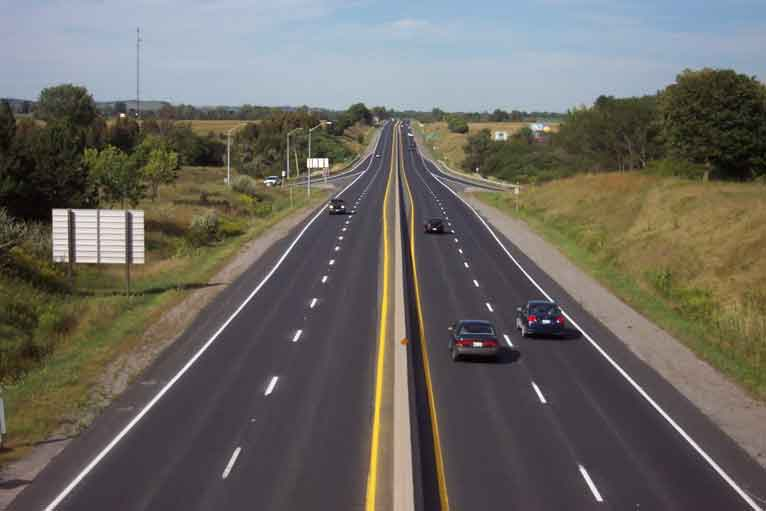
\includegraphics[scale=0.14]{images/highway.jpg}
\captionof{figure}{Autoroute}
\end{minipage}%
\begin{minipage}{.4\textwidth}
\centering
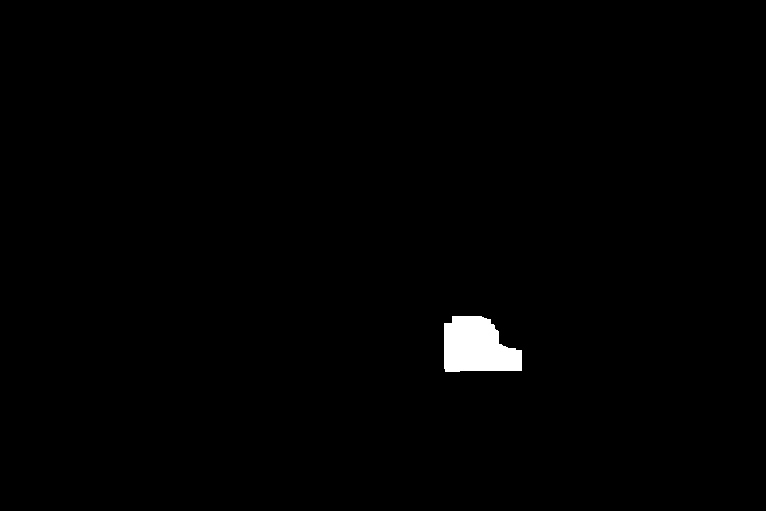
\includegraphics[scale=0.14]{highway-mask.png}
\captionof{figure}{Masque appliqué}
\end{minipage}%
\begin{minipage}{.4\textwidth}
\centering
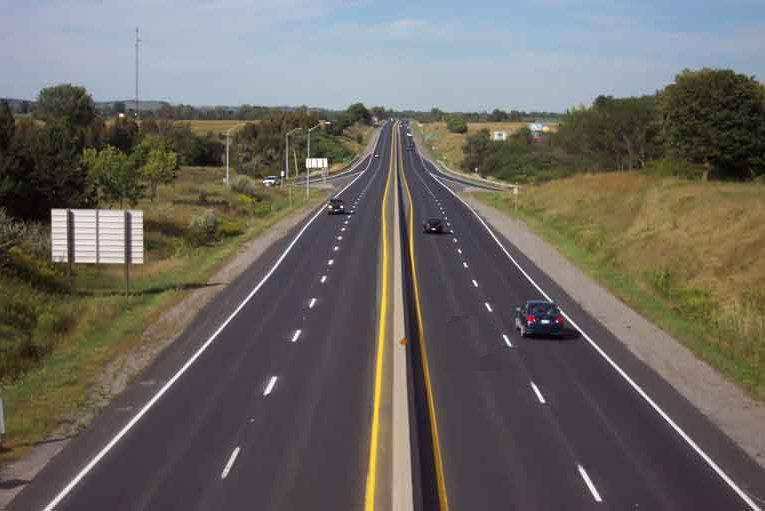
\includegraphics[scale=0.14]{inpainted_highway17.png}
\captionof{figure}{patchsize=17}
\end{minipage}%
\end{figure}

\begin{figure}[H]
\begin{minipage}{.4\textwidth}
\centering
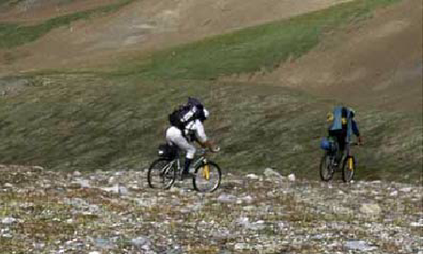
\includegraphics[scale=0.25]{images/bike.png}
\captionof{figure}{Vélos}
\end{minipage}%
\begin{minipage}{.4\textwidth}
\centering
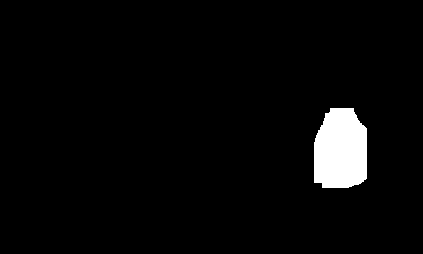
\includegraphics[scale=0.25]{bike_mask17.png}
\captionof{figure}{Masque appliqué}
\end{minipage}%
\begin{minipage}{.4\textwidth}
\centering
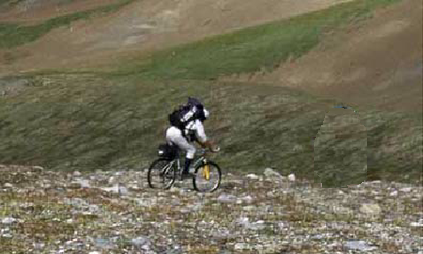
\includegraphics[scale=0.25]{inpainted_bike17.png}
\captionof{figure}{patchsize=17}
\end{minipage}%
\end{figure}

\begin{figure}[H]
\begin{minipage}{.4\textwidth}
\centering
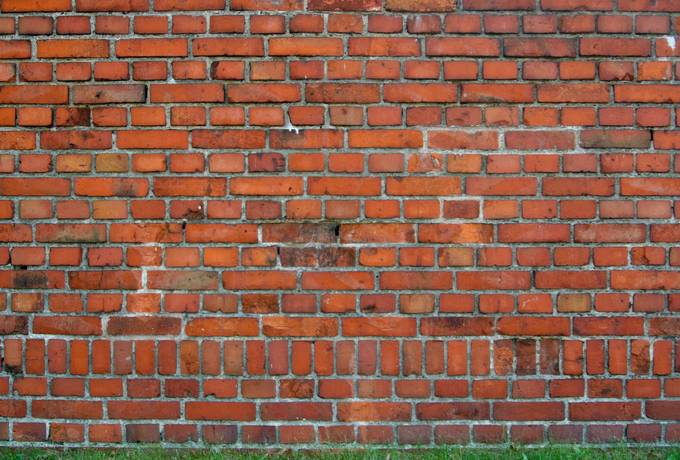
\includegraphics[scale=0.15]{images/wall3.jpg}
\captionof{figure}{Mur}
\end{minipage}%
\begin{minipage}{.4\textwidth}
\centering
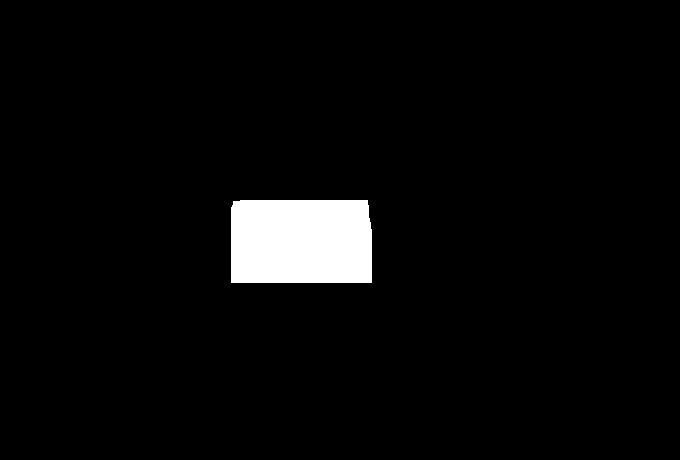
\includegraphics[scale=0.15]{mask_wall3_29.png}
\captionof{figure}{Masque appliqué}
\end{minipage}%
\begin{minipage}{.4\textwidth}
\centering
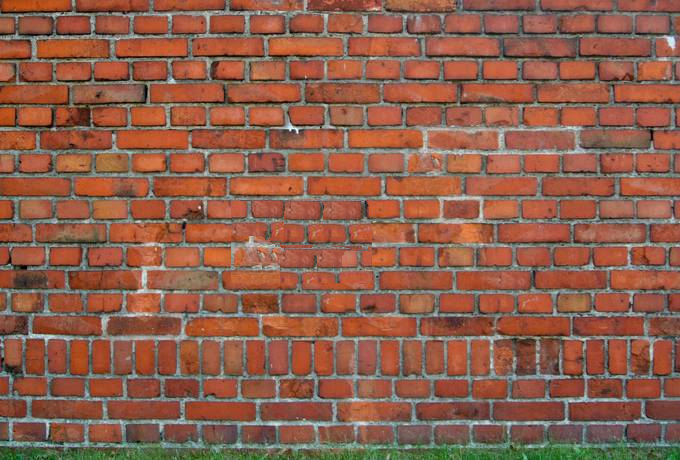
\includegraphics[scale=0.15]{wall3_inpainted29.png}
\captionof{figure}{patchsize=29}
\end{minipage}%
\end{figure}

\begin{figure}[H]
\begin{minipage}{.4\textwidth}
\centering
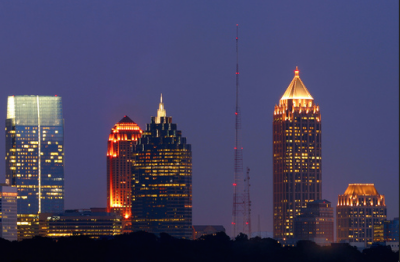
\includegraphics[scale=0.25]{images/skyline.png}
\captionof{figure}{Buildings}
\end{minipage}%
\begin{minipage}{.4\textwidth}
\centering
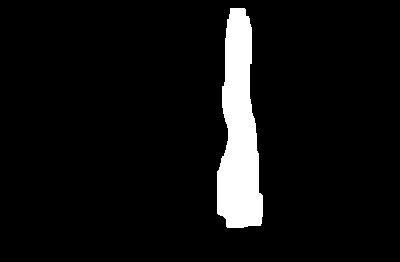
\includegraphics[scale=0.25]{skyline-mask.png}
\captionof{figure}{Masque appliqué}
\end{minipage}%
\begin{minipage}{.4\textwidth}
\centering
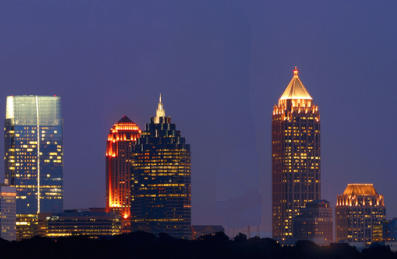
\includegraphics[scale=0.25]{inpainted_skyline17.png}
\captionof{figure}{patchsize=17}
\end{minipage}%
\end{figure}

\begin{figure}[H]
\begin{minipage}{.4\textwidth}
\centering
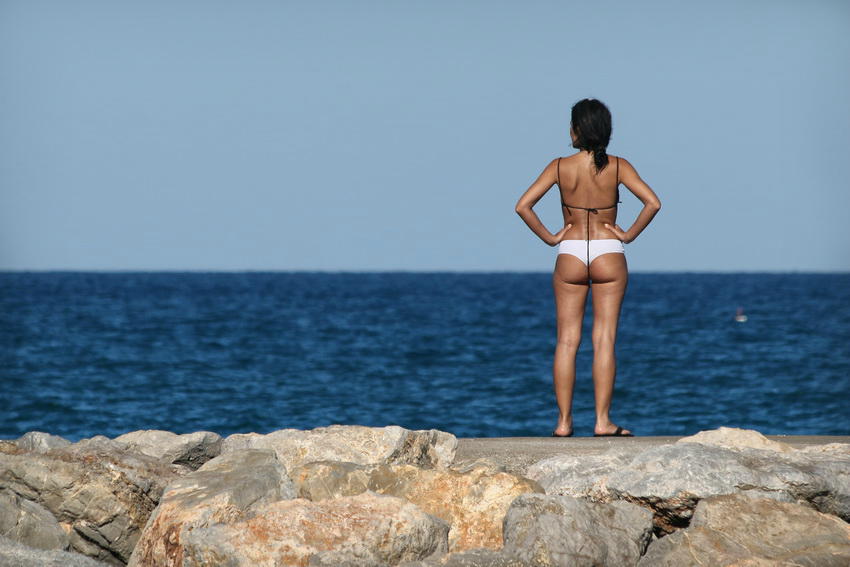
\includegraphics[scale=0.15]{images/women.png}
\captionof{figure}{Femme devant la mer}
\end{minipage}%
\begin{minipage}{.4\textwidth}
\centering
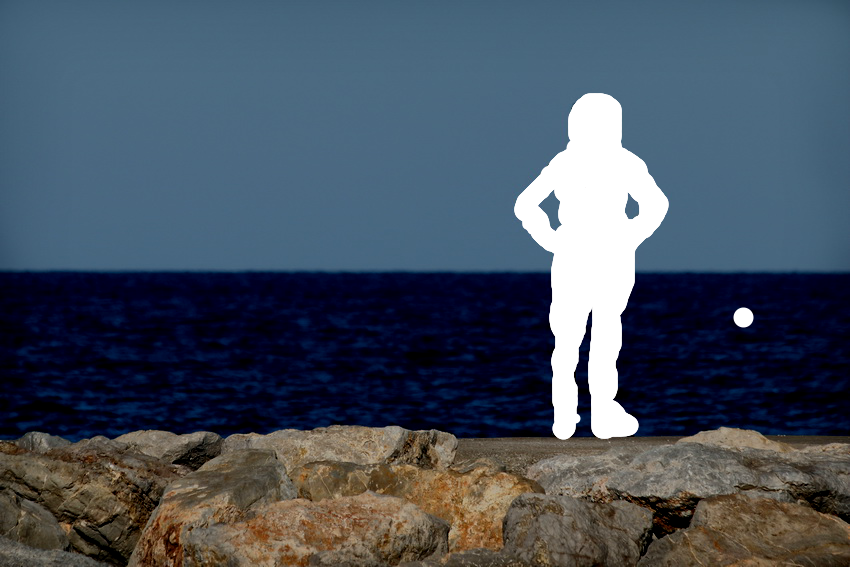
\includegraphics[scale=0.15]{images/women-mask.png}
\captionof{figure}{Masque appliqué}
\end{minipage}%
\begin{minipage}{.4\textwidth}
\centering
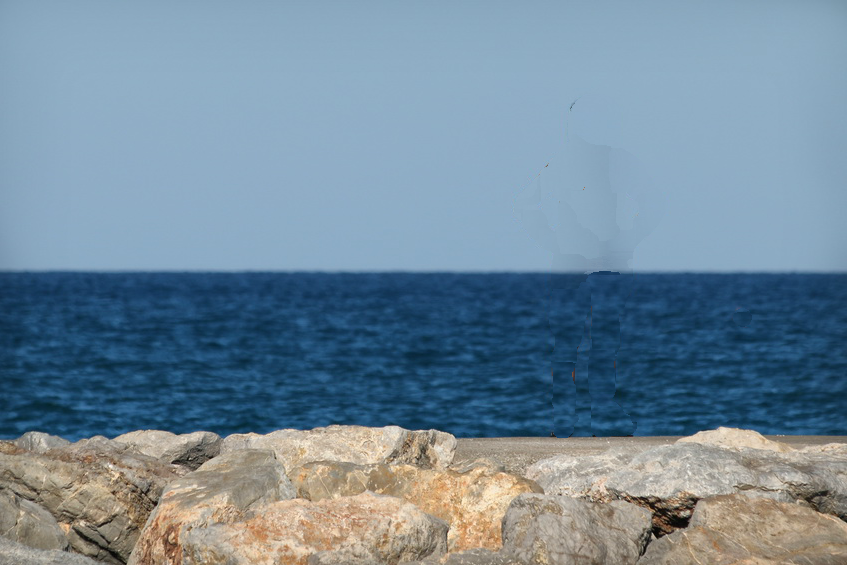
\includegraphics[scale=0.15]{inpainted_women27.png}
\captionof{figure}{patchsize=27}
\end{minipage}%
\end{figure}

\begin{figure}[H]
\begin{minipage}{.4\textwidth}
\centering
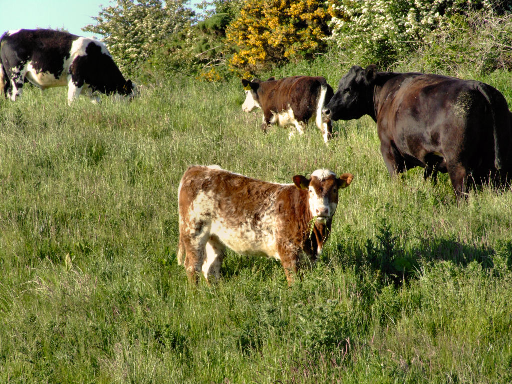
\includegraphics[scale=0.25]{images/cow.png}
\captionof{figure}{Vaches}
\end{minipage}%
\begin{minipage}{.4\textwidth}
\centering
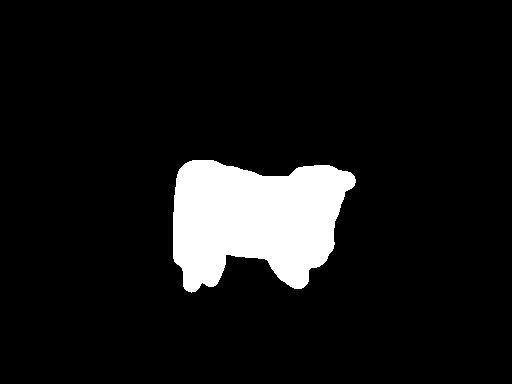
\includegraphics[scale=0.25]{images/cow-mask.png}
\captionof{figure}{Masque appliqué}
\end{minipage}%
\begin{minipage}{.4\textwidth}
\centering
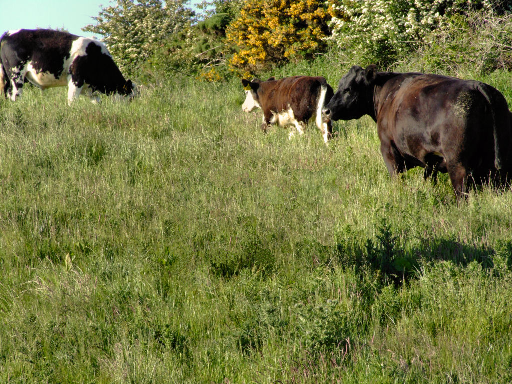
\includegraphics[scale=0.25]{inpainted/perfect-cow.png}
\captionof{figure}{patchsize=7}
\end{minipage}%
\end{figure}

\begin{figure}[H]
\begin{minipage}{.4\textwidth}
\centering
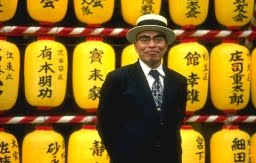
\includegraphics[scale=0.45]{images/asiatic.jpg}
\captionof{figure}{Homme devant des lampions}
\end{minipage}%
\begin{minipage}{.4\textwidth}
\centering

\includegraphics[scale=0.45]{images/asiatic_mask.png}
\captionof{figure}{Masque appliqué}
\end{minipage}%
\begin{minipage}{.4\textwidth}
\centering
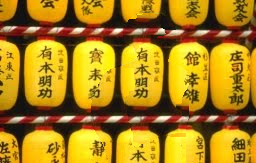
\includegraphics[scale=0.53]{inpainted/bench_asiatique29.png}
\captionof{figure}{patchsize=29}
\end{minipage}%
\end{figure}

\begin{figure}[H]
\begin{minipage}{.4\textwidth}
\centering
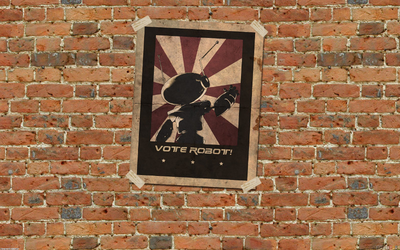
\includegraphics[scale=0.35]{images/wall.png}
\captionof{figure}{Homme devant des lampions}
\end{minipage}%
\begin{minipage}{.4\textwidth}
\centering

\includegraphics[scale=0.35]{images/wall_mask.png}
\captionof{figure}{Masque appliqué}
\end{minipage}%
\begin{minipage}{.4\textwidth}
\centering
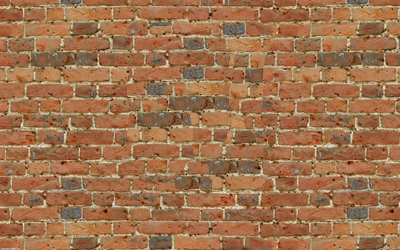
\includegraphics[scale=0.4]{bench_wall17.png}
\captionof{figure}{patchsize=17}
\end{minipage}%
\end{figure}

\subsection{Echecs}

\begin{figure}[H]
\begin{minipage}{.4\textwidth}
\centering
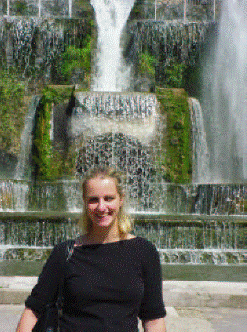
\includegraphics[scale=0.3]{images/girl.png}
\captionof{figure}{Femme devant la fontaine}
\end{minipage}%
\begin{minipage}{.4\textwidth}
\centering
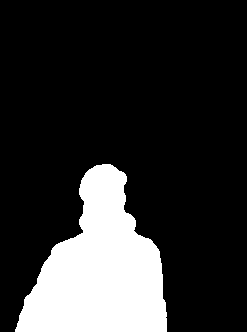
\includegraphics[scale=0.3]{images/girl_mask.png}
\captionof{figure}{Masque appliqué}
\end{minipage}%
\begin{minipage}{.4\textwidth}
\centering
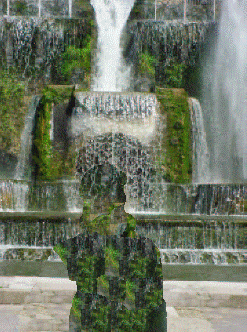
\includegraphics[scale=0.36]{bench_girl19.png}
\captionof{figure}{patchsize=19}
\end{minipage}%
\end{figure}

\begin{figure}[H]
\begin{minipage}{.4\textwidth}
\centering
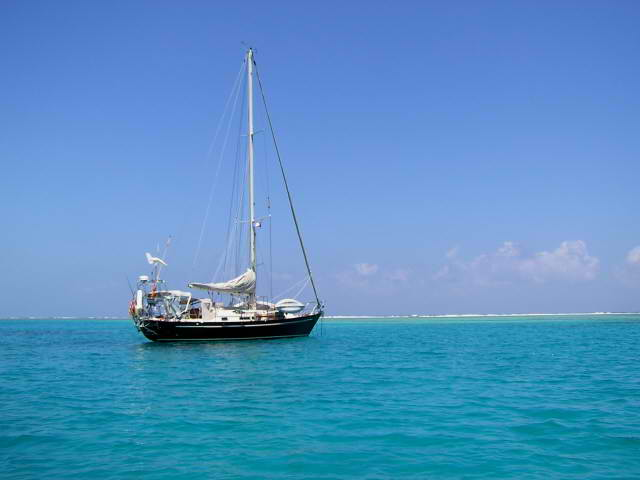
\includegraphics[scale=0.18]{images/boat.jpg}
\captionof{figure}{Bateau}
\end{minipage}%
\begin{minipage}{.4\textwidth}
\centering
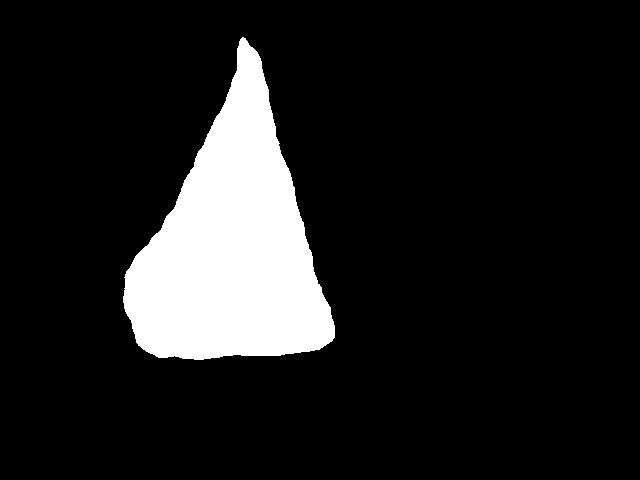
\includegraphics[scale=0.18]{images/boat_mask.png}
\captionof{figure}{Masque appliqué}
\end{minipage}%
\begin{minipage}{.4\textwidth}
\centering
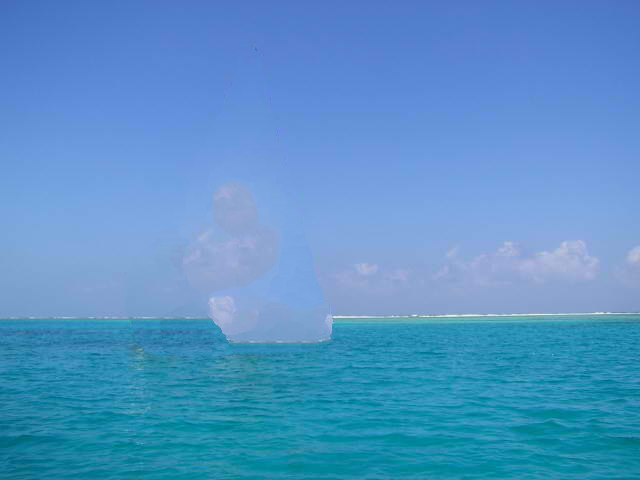
\includegraphics[scale=0.22]{bench_boat9.png}
\captionof{figure}{patchsize=9}
\end{minipage}%
\end{figure}

\begin{figure}[H]
\begin{minipage}{.4\textwidth}
\centering
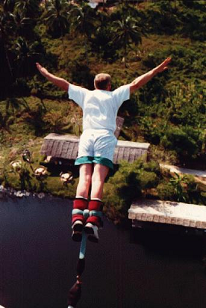
\includegraphics[scale=0.23]{images/bungee.png}
\captionof{figure}{Saut}
\end{minipage}%
\begin{minipage}{.4\textwidth}
\centering
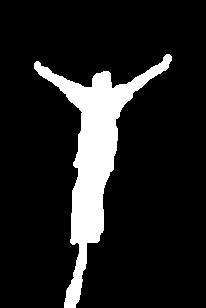
\includegraphics[scale=0.23]{images/bungee-mask.png}
\captionof{figure}{Masque appliqué}
\end{minipage}%
\begin{minipage}{.4\textwidth}
\centering
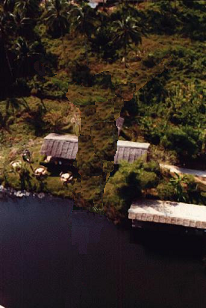
\includegraphics[scale=0.35]{bench_bungee17.png}
\captionof{figure}{patchsize=17}
\end{minipage}%
\end{figure}

\begin{figure}[H]
\begin{minipage}{.4\textwidth}
\centering
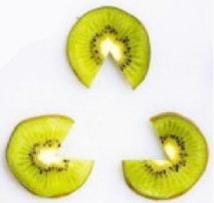
\includegraphics[scale=0.23]{images/kiwi.png}
\captionof{figure}{Saut}
\end{minipage}%
\begin{minipage}{.4\textwidth}
\centering

\includegraphics[scale=0.23]{images/kiwi_mask.png}
\captionof{figure}{Masque appliqué}
\end{minipage}%
\begin{minipage}{.4\textwidth}
\centering
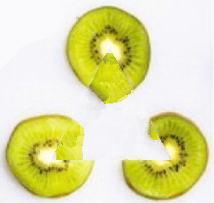
\includegraphics[scale=0.35]{bench_kiwi9.png}
\captionof{figure}{patchsize=9}
\end{minipage}%
\end{figure}
\end{document}
